\documentclass{article}%
\usepackage{amsmath}
\usepackage{graphicx}
\usepackage{amsfonts}%
\usepackage{amssymb}


\setlength{\topmargin}{-0.75in}
\setlength{\textheight}{9.25in}
\setlength{\oddsidemargin}{0.0in}
\setlength{\evensidemargin}{0.0in}
\setlength{\textwidth}{6.5in}
\def\labelenumi{\arabic{enumi}.}
\def\theenumi{\arabic{enumi}}
\def\labelenumii{(\alph{enumii})}
\def\theenumii{\alph{enumii}}
\def\p@enumii{\theenumi.}
\def\labelenumiii{\arabic{enumiii}.}
\def\theenumiii{\arabic{enumiii}}
\def\p@enumiii{(\theenumi)(\theenumii)}
\def\labelenumiv{\arabic{enumiv}.}
\def\theenumiv{\arabic{enumiv}}
\def\p@enumiv{\p@enumiii.\theenumiii}
\pagestyle{plain}
\setcounter{secnumdepth}{0}
\newtheorem{theorem}{Theorem}
\newtheorem{acknowledgement}[theorem]{Acknowledgement}
\newtheorem{algorithm}[theorem]{Algorithm}
\newtheorem{axiom}[theorem]{Axiom}
\newtheorem{case}[theorem]{Case}
\newtheorem{claim}[theorem]{Claim}
\newtheorem{conclusion}[theorem]{Conclusion}
\newtheorem{condition}[theorem]{Condition}
\newtheorem{conjecture}[theorem]{Conjecture}
\newtheorem{corollary}[theorem]{Corollary}
\newtheorem{criterion}[theorem]{Criterion}
\newtheorem{definition}[theorem]{Definition}
\newtheorem{example}[theorem]{Example}
\newtheorem{exercise}[theorem]{Exercise}
\newtheorem{lemma}[theorem]{Lemma}
\newtheorem{notation}[theorem]{Notation}
\newtheorem{problem}[theorem]{Problem}
\newtheorem{proposition}[theorem]{Proposition}
\newtheorem{remark}[theorem]{Remark}
\newtheorem{solution}[theorem]{Solution}
\newtheorem{summary}[theorem]{Summary}
\newenvironment{proof}[1][Proof]{\textbf{#1.} }{\ \rule{0.5em}{0.5em}}

\begin{document}

\title{Interpretable Machine Learning, Assignment 1}
\author{Chuan Lu}
\date{February 5, 2020}
\maketitle

\newcommand{\hxi}{\hat{x}_i}
\newcommand{\hw}{\hat{w}}

Code for this Assignment are contained in \texttt{optimizer.py} (algorithms), and \texttt{Assignment1.ipynb} (main process).

\begin{enumerate}

\item Problem 1.a and Problem 2.(a)

Let $x_i, w\in\mathbb{R}^d $, and $\hxi = (1, x_i^\top)^\top ,\hw = (w_0, w^\top)^\top \in\mathbb{R}^{d+1} $. Denote
\begin{equation}
p(y = 1\mid \hxi) = \sigma(\hxi)
\end{equation}
then the loss function of logistic regression is
\begin{equation}
\begin{aligned}
\mathcal{L} &= -\sum_{i=1}^{n}\Big ( y_i \log p(y = 1 \mid \hxi) + (1-y_i)\log (1- p(y = 1 \mid \hxi)\Big ) \\
&= -\sum_{i=1}^{n} \Big( y_i \log\sigma(\hxi) + (1-y_i)\log(1-\sigma(\hxi))\Big),
\end{aligned}
\end{equation}

and the gradient is
\begin{equation}
\begin{aligned}
\frac{\partial}{\partial \hw}\mathcal{L} &= -\sum_{i=1}^{n} \Big( \frac{y_i}{\sigma(\hxi)}\frac{\partial \sigma}{\partial \hw}(\hxi) - \frac{1-y_i}{1-\sigma(\hxi)}\frac{\partial \sigma}{\partial \hw}(\hxi)\Big) \\
&= \sum_{i=1}^{n}\frac{\sigma(\hxi)-y_i}{\sigma(\hxi)(1-\sigma(\hxi))}\frac{\partial \sigma}{\partial \hw}(\hxi).
\end{aligned}
\end{equation}

Notice that
\begin{equation}
\begin{aligned}
\frac{\partial \sigma}{\partial \hw}(\hxi) &= \frac{\partial}{\partial \hw}\frac{1}{1+e^{-\hxi^\top \hw}} = \frac{\hxi e^{-\hxi^\top \hw}}{(1+e^{-\hxi^\top \hw)^2}} = \sigma(\hxi)(1-\sigma(\hxi))\hxi,
\end{aligned}
\end{equation}

then
\begin{equation}
\begin{aligned}
\frac{\partial}{\partial \hw}\mathcal{L} &= \sum_{i=1}^{n}(\sigma(\hxi)-y_i)\hxi.
\end{aligned}
\end{equation}

The code for the gradient descent algorithm is in \texttt{optimizer.py}. In the implementations, we use the mean of losses for each sample instead of the sum, for a fair comparison between the training loss and test loss. The coefficients $\hw$ are initialized as zeros, and we use learning rate $lr = 0.01$ in training. The convergence plot is shown in Figure \ref{problem1a-convergence}.

\begin{figure}[htbp]
\centering
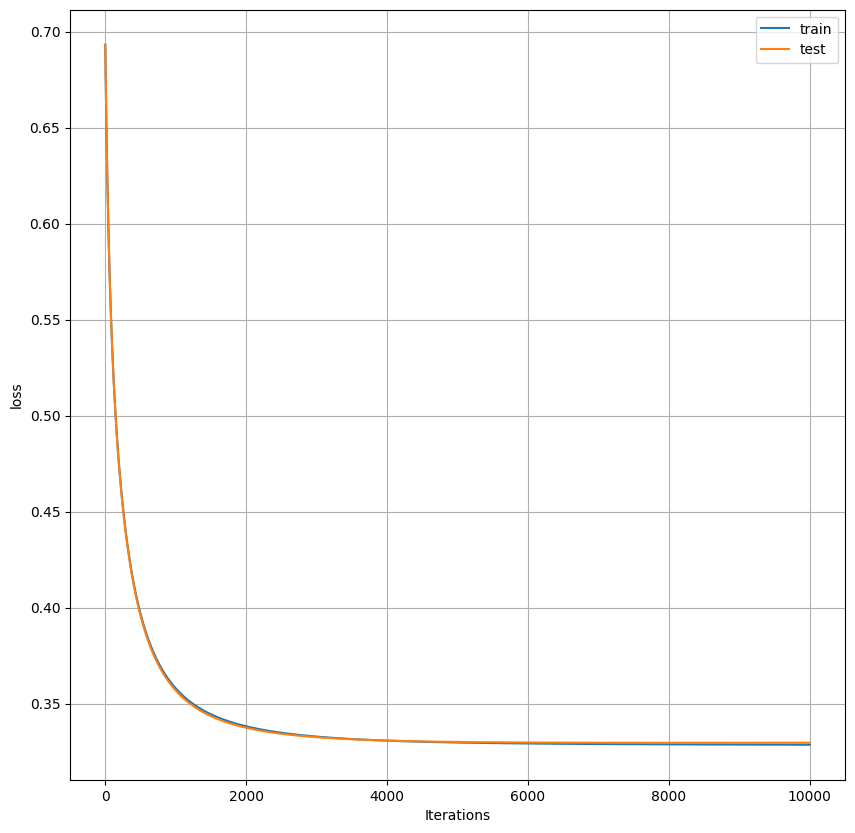
\includegraphics[scale=0.4]{problem1a.png}
\caption{Convergence of loss v.s. number of iterations for Problem 1a, using gradient descent. The orange line shows the test loss, and the blue line represents the training loss.}
\label{problem1a-convergence}
\end{figure}

The ROC-AUC and precision-recall curve on the test set is reported in Figure \ref{problem1a-metric}. The F1-score is 0.6476.

\begin{figure}[htbp]
\centering
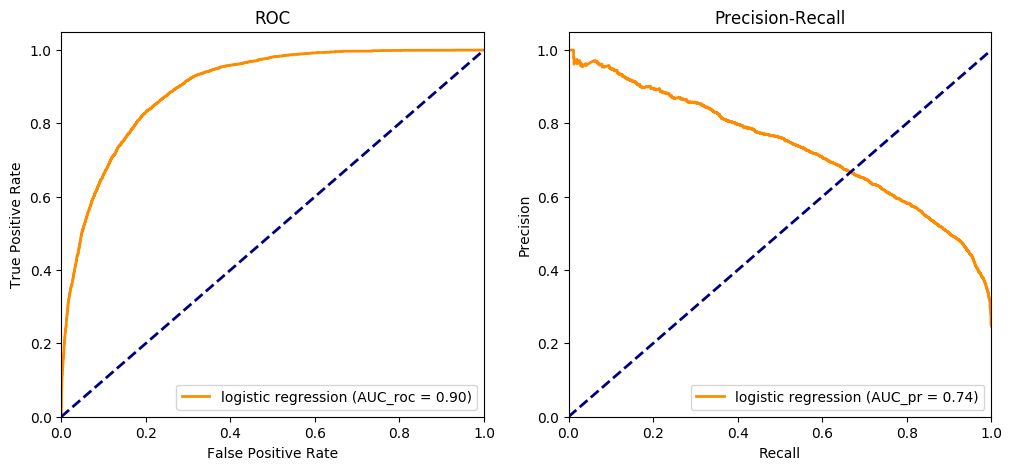
\includegraphics[scale=0.5]{problem1a_metric.png}
\caption{ROC, precision-recall curve, AUC for Problem 1.a (GD-solved logistic regression).}
\label{problem1a-metric}
\end{figure}

\item Problem 1.b and Problem 2.(b)

The code for simulated annealing is in \texttt{optimizer.py}. For this problem, we use the same preprocessing process with Problem 1.a. We use a linearly decreasing scheduler for temperature, and the weights $\hw$ are initialized with zeros. 
The convergence plot is shown in Figure \ref{problem1b-convergence}. 

\begin{figure}[htbp]
\centering
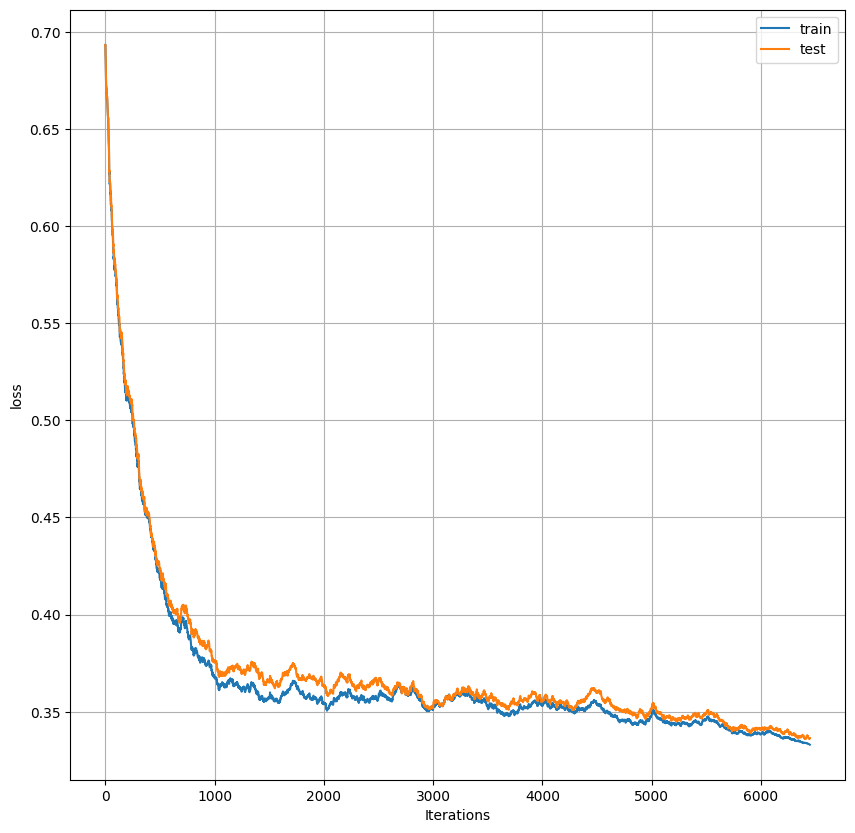
\includegraphics[scale=0.4]{problem1b.png}
\caption{Convergence of loss v.s. number of iterations for Problem 1b, using simulated annealing. The orange line shows the test loss, and the blue line represents the training loss.}
\label{problem1b-convergence}
\end{figure}

The ROC-AUC and precision-recall curve on the test set is reported in Figure \ref{problem1a-metric}. The F1-score is 0.6415.

\begin{figure}[htbp]
\centering
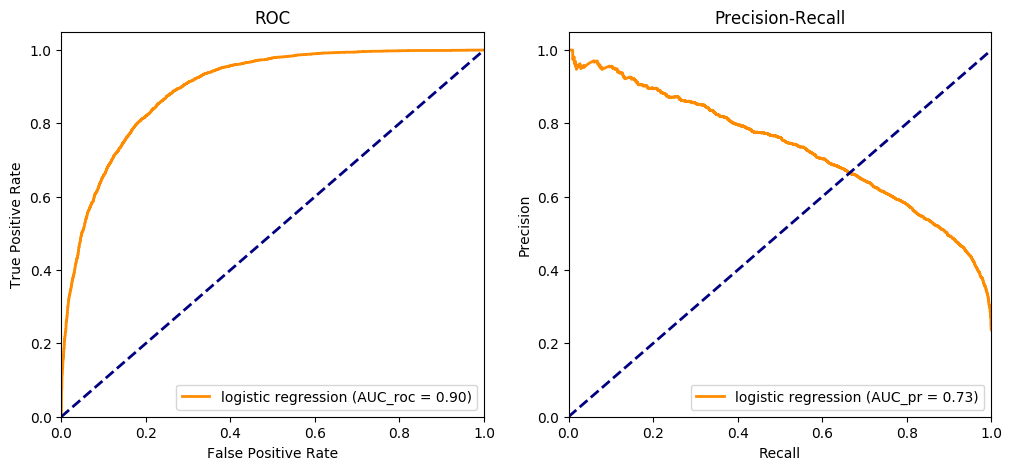
\includegraphics[scale=0.5]{problem1b_metric.png}
\caption{ROC, precision-recall curve, AUC for Problem 1.b (SA-solved logistic regression).}
\label{problem1b-metric}
\end{figure}


\item Problem 3

We use the same preprocessing process as in Problem 1.a. 

The ROC and AUC are shown in Figure \ref{problem3}. Although ROC, AUC of Lasso are very similar with logistic regression, the number of non-zero coefficients is 17 instead of 89 for both solutions of logistic regression. This comes from the $L_1 $ penalty of lasso, while logistic regression does not have any penalty on the number of non-zero coefficients.

\begin{figure}[htbp]
\centering
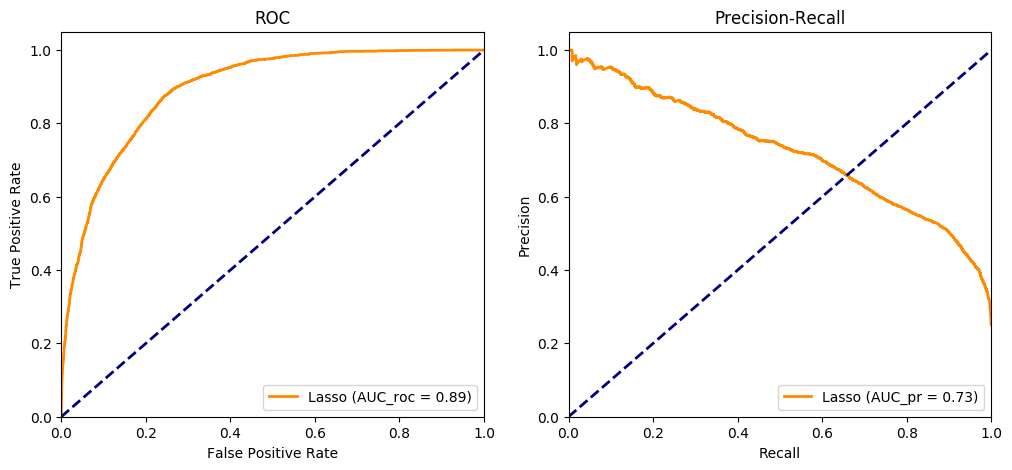
\includegraphics[scale=0.5]{problem3.png}
\caption{ROC and AUC for Problem 3 (Lasso).}
\label{problem3}
\end{figure}

\item Problem 4

For this problem, we still use the same preprocessing process as in Problem 1.a. 

The feature importance plot for the 20 most important features is shown in Figure \ref{problem4-importance}.

\begin{figure}[htbp]
\centering
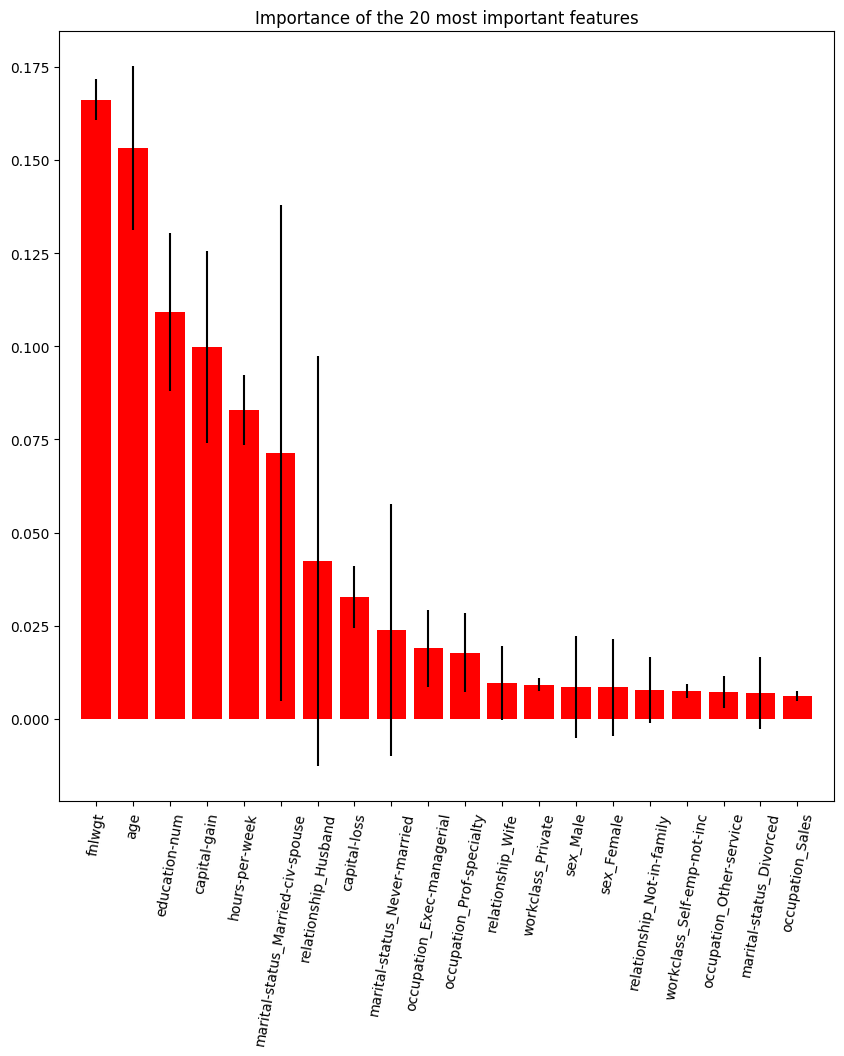
\includegraphics[scale=0.5]{problem4_importance.png}
\caption{Feature importance for Problem 4 (Random Forest).}
\label{problem4-importance}
\end{figure}

The absolute value of weights (and corresponding rank) of each features are mostly consistent with the importance in Random Forest, with an exception \texttt{fnlwgt}, which is the most important in Random Forest but has less weights in logistic regression. 

\end{enumerate}


\end{document}